\documentclass[12pt, letterpaper, onecolumn]{article}
\usepackage[utf8]{inputenc}
\usepackage[english]{babel}
\usepackage[textwidth=16cm]{geometry}
\usepackage{pdfpages}
\usepackage{amssymb}
\usepackage{graphicx}
\usepackage{setspace}
\usepackage{nicefrac}
\usepackage{hyperref}
\usepackage{pgfplots}
\usepackage{grffile}
\usepackage{amsmath}
\usepackage{commath}
\usepackage{siunitx}
\usepackage{float}

\pgfplotsset{compat=newest}
\usetikzlibrary{plotmarks}
\usetikzlibrary{arrows.meta}
\usepgfplotslibrary{patchplots}
\NewDocumentCommand{\codeword}{v}{% 
\texttt{#1}}%
\DeclareMathOperator{\Span}{span}

\title{Project 2 - MECH 7790}
\author{Andrew Weir, Tanner Koza}
\date\today

\begin{document}
\maketitle

\section*{Part II: Group Portion}

\subsection*{Problem 3: LQR State Feedback Regulation}

\subsubsection*{a) Design the controller for the linear model.}

$Q$, $R$, and $K$ were designed using the following methodology. $Q$ was designed using Bryson's rule to unit scale the max $\theta$ requirement of 0.61 rad and an arbitrary maximum $x$ (set at 0.55 m) to limit overshoot. The derivatives of the states in question were set to a value of 1 as their weighting is inherently captured within the $\theta$ and $x$ states.

\begin{equation*}
    \begin{split}
        Q & =
        \begin{bmatrix}
            3.31 & 0 & 0    & 0 \\
            0    & 1 & 0    & 0 \\
            0    & 0 & 2.69 & 0 \\
            0    & 0 & 0    & 1 \\
        \end{bmatrix}
    \end{split}
\end{equation*}

$R$ was set to a value of 1 as there is only 1 input, meaning there is more value in scaling $Q$ relative to $R$ given the performance of your LQR controller is determined by the ratio between the two.

Using \codeword{icare()} in MATLAB, the controller $K$ was determined to be the following:

\begin{equation*}
    \begin{split}
        K & =
        \begin{bmatrix}
            -1.82 & -2.70 & 22.32 & 4.30 \\
        \end{bmatrix}
    \end{split}
\end{equation*}\

\codeword{icare()} solves the Algebraic Riccati Equation ($A^TP +  PA + Q -PBR^{-1}B^TP = 0$) for $P$ which is used in determining the controller $K$ with the following:

\begin{equation*}
    \begin{split}
        K & = R^{-1}B^TP
    \end{split}
\end{equation*}

The following figures depict the outputs and input of the linear system with the above controller:

\begin{figure}[!ht]
    \centering
    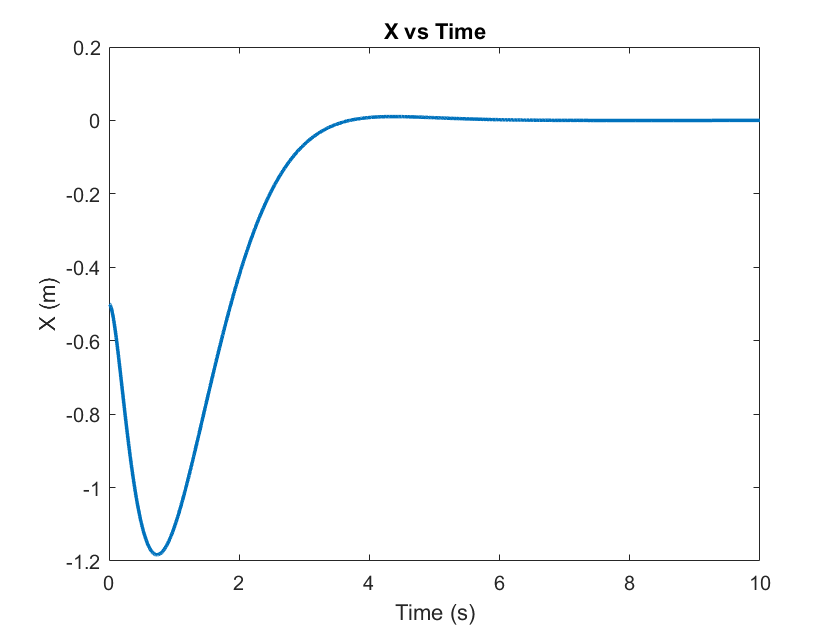
\includegraphics[width=\linewidth]{figs/sf_lin_x.png}
    \caption{Linear System X Output}
    \label{}
\end{figure}

\begin{figure}[!ht]
    \centering
    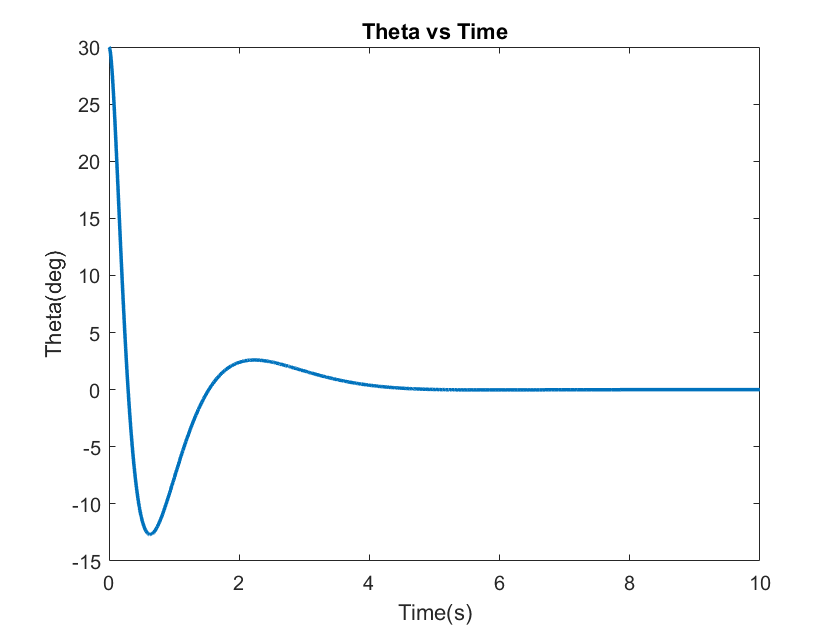
\includegraphics[width=\linewidth]{figs/sf_lin_theta.png}
    \caption{Linear System $\theta$ Output}
    \label{}
\end{figure}

\begin{figure}[!ht]
    \centering
    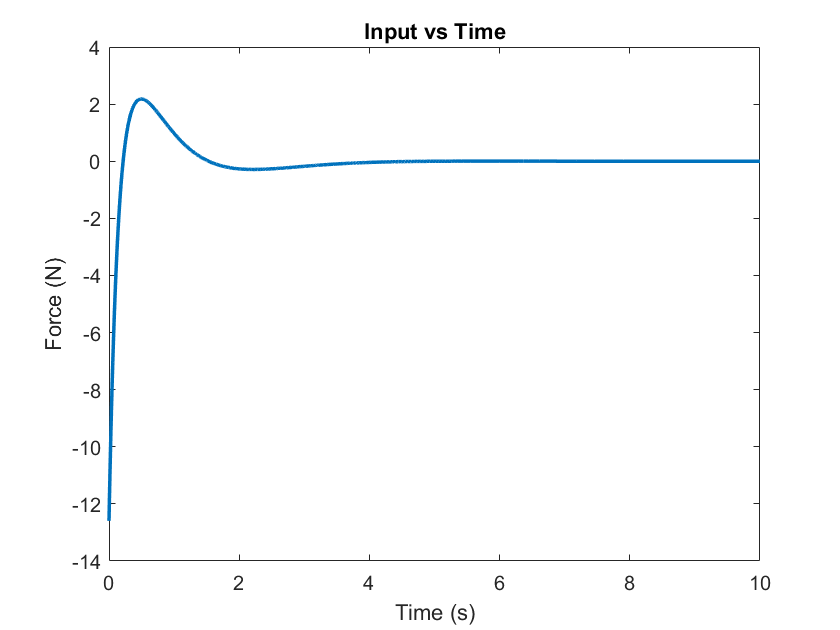
\includegraphics[width=\linewidth]{figs/sf_lin_input.png}
    \caption{Linear System Input}
    \label{}
\end{figure}

\clearpage

The closed-loop eigenvalues are also found in the result of \codeword{icare()}, but it is simply from $det(sI-(A-BK))=0$. They are the following:

\begin{equation*}
    \begin{split}
        s & = -1.32\pm0.88, -3.85, -8.34
    \end{split}
\end{equation*}

\subsubsection*{b) Design the controller for the nonlinear model.}

The $Q$, $R$, and $K$ used for the nonlinear system are the same as for the linear model.

The following figures depict the outputs and input of the nonlinear system with the above controller:

\begin{figure}[!ht]
    \centering
    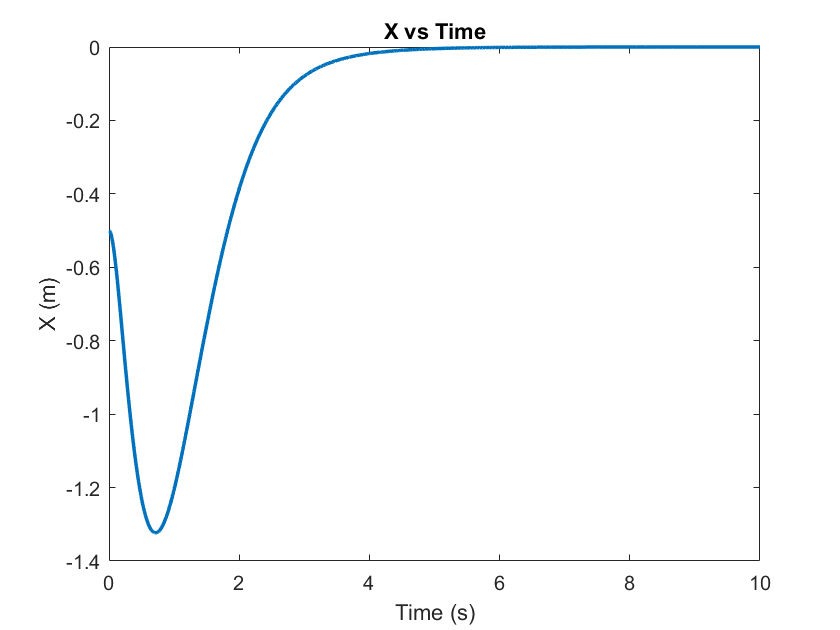
\includegraphics[width=\linewidth]{figs/sf_nlin_x.png}
    \caption{Nonlinear System X Output}
    \label{}
\end{figure}

\begin{figure}[!ht]
    \centering
    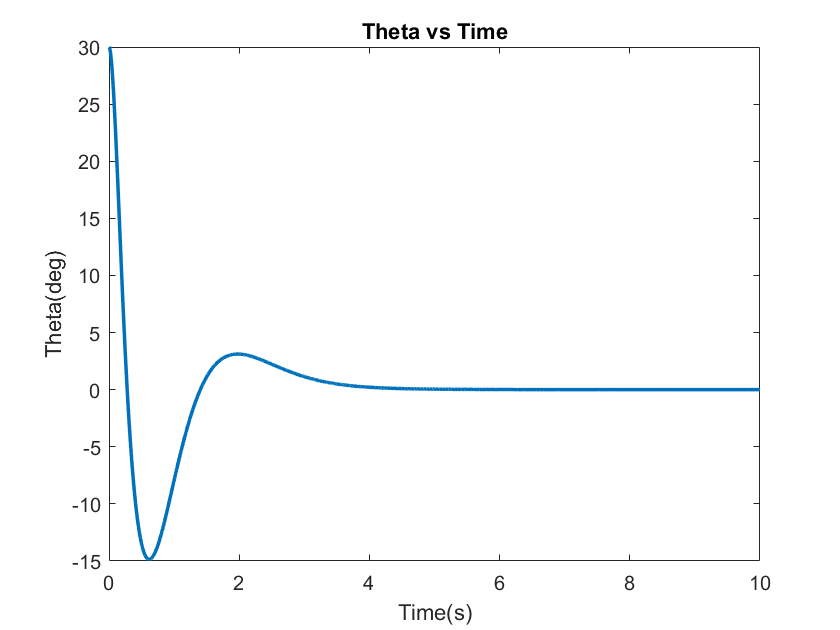
\includegraphics[width=\linewidth]{figs/sf_nlin_theta.png}
    \caption{Nonlinear System $\theta$ Output}
    \label{}
\end{figure}

\begin{figure}[!ht]
    \centering
    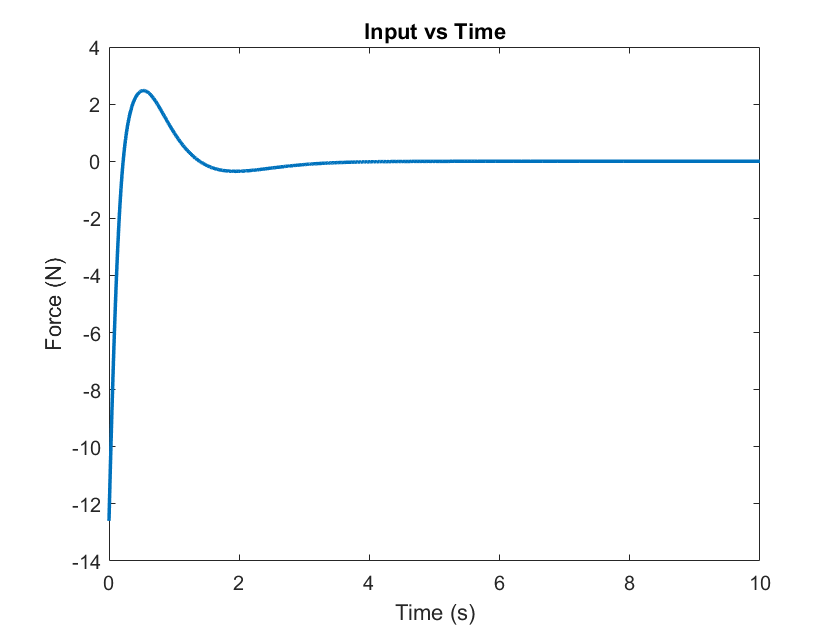
\includegraphics[width=\linewidth]{figs/sf_nlin_input.png}
    \caption{Nonlinear System Input}
    \label{}
\end{figure}

\subsubsection*{c) Discuss the differences between tuning the model for the linear and nonlinear model.}

For our particular case, there was no difference in tuning as the $Q$ and $R$ values for the linear model were able to produce a $K$ that yielded stable results that met the design requirements for the nonlinear model. The settling time of the nonlinear response is slightly slower than that for the linear model as expected, but it is still within the performance requirements. If our initial tune was not successful, we would have likely needed to increase our values within $Q$ to account for the nonlinear dynamics.

\clearpage
\subsection*{Problem 4: LQR State Feedback Regulation}

The following table outlines the 5 different combinations of $Q$ and $R$ with the corresponding $K$ we tested on the linear model. The values for $Q$ in the table indicate the diagonal terms with the off-diagonal terms being 0. The $Q$ for Combination 1 was derived using $Q = C^TQ_1C$.

\begin{table}[!ht]
    \centering
    \caption{Q $\&$ R Combinations with Resulting K $\&$ s}
    \begin{tabular}{|*5{c|}}
        \hline
        $\#$ & $Q$                                                                           & $R$ & $K$                                                           & $s$                                                             \\ [0.5ex]
        \hline
        1    & $diag\left(\begin{bmatrix}3.31 \\ 0  \\ 2.69 \\ 0 \end{bmatrix}\right)$       & 1   & $\begin{bmatrix} -1.82 & -2.38 & 20.85 & 3.89 \end{bmatrix}$  & $\begin{array}{cc} -1.14\pm1.11 \\ -5.62\pm0.67 \end{array}$    \\
        \hline
        2    & $diag\left(\begin{bmatrix}33.06 \\ 10  \\ 26.87 \\ 10 \end{bmatrix}\right)$   & 1   & $\begin{bmatrix} -5.75 & -6.92 & 38.02  & 7.96 \end{bmatrix}$ & $\begin{array}{cc} -1.96 \\ -2.37\pm1.44 \\  -17.07\end{array}$ \\
        \hline
        3    & $diag\left(\begin{bmatrix}3.31 \\ 1  \\ 2.69 \\ 1 \end{bmatrix}\right)$       & 10  & $\begin{bmatrix} -0.58 & -1.27 & 17.57 & 3.25 \end{bmatrix}$  & $\begin{array}{cc} -0.68\pm0.59 \\ -4.95 \\  -6.33\end{array}$  \\
        \hline
        4    & $diag\left(\begin{bmatrix}3.31 \\ 1  \\ 2.69 \\ 1 \end{bmatrix}\right)$       & 1   & $\begin{bmatrix} -1.82 & -2.70 & 22.32 & 4.30  \end{bmatrix}$ & $\begin{array}{cc} -1.32\pm0.88 \\  -3.85 \\ -8.34\end{array}$  \\
        \hline
        5    & $diag\left(\begin{bmatrix}0.17 \\ 0.05  \\ 0.13 \\ 0.05 \end{bmatrix}\right)$ & 1   & $\begin{bmatrix} -0.41 & -1.04 & 16.84 & 3.10  \end{bmatrix}$ & $\begin{array}{cc} -0.57\pm0.51 \\  -5.13 \\ -6.10\end{array}$  \\
        \hline
    \end{tabular}
\end{table}

\clearpage

The following figures depict the outputs and input of the linear system with the above controllers from the 5 combinations:

\begin{figure}[!ht]
    \centering
    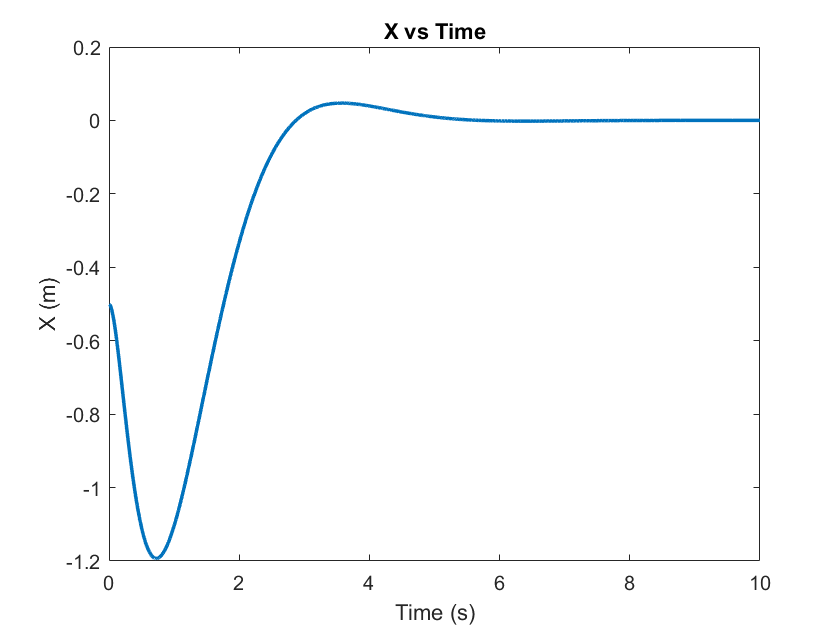
\includegraphics[width=\linewidth]{figs/sf_lin_c1_x.png}
    \caption{Combination $\#$1 - Linear System X Output}
    \label{}
\end{figure}

\begin{figure}[!ht]
    \centering
    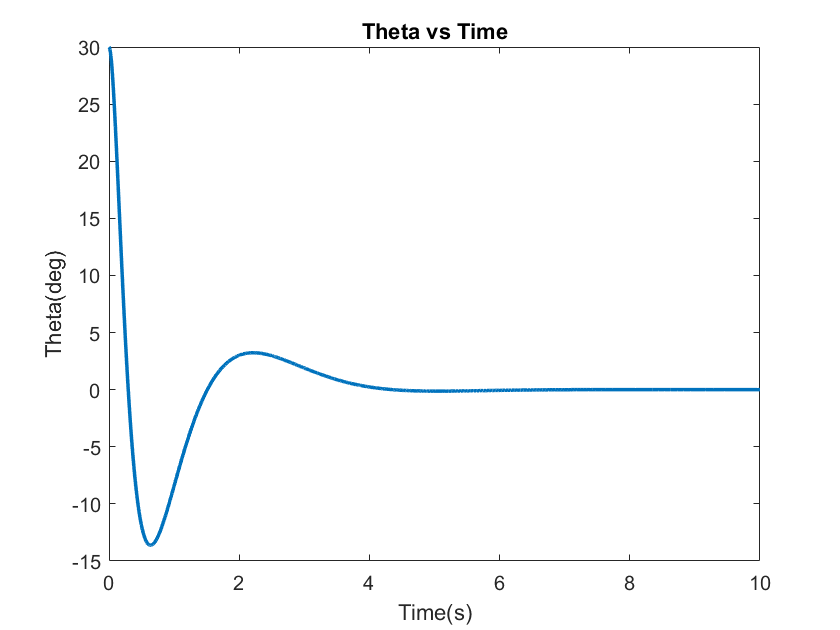
\includegraphics[width=\linewidth]{figs/sf_lin_c1_theta.png}
    \caption{Combination $\#$1 - Linear System $\theta$ Output}
    \label{}
\end{figure}

\begin{figure}[!ht]
    \centering
    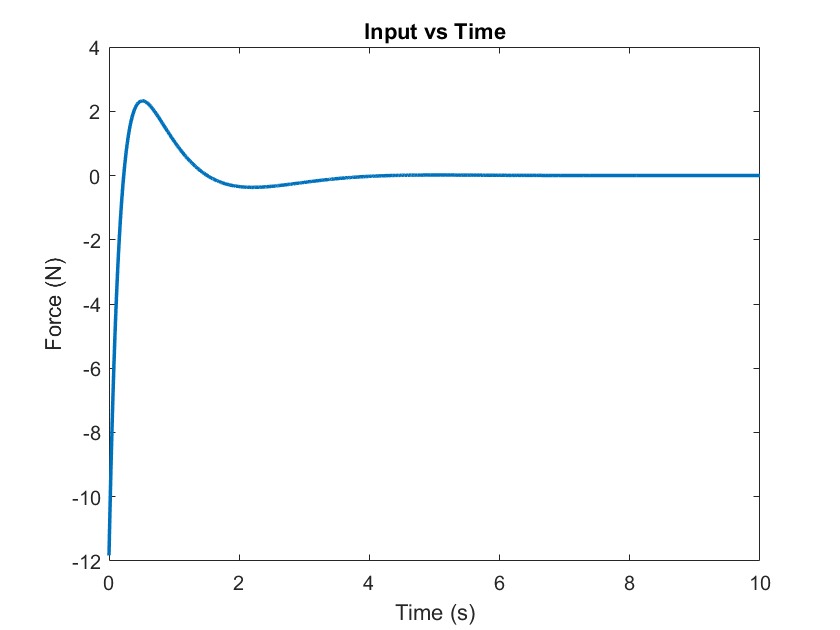
\includegraphics[width=\linewidth]{figs/sf_lin_c1_input.png}
    \caption{Combination $\#$1 - Linear System Input}
    \label{}
\end{figure}

\begin{figure}[!ht]
    \centering
    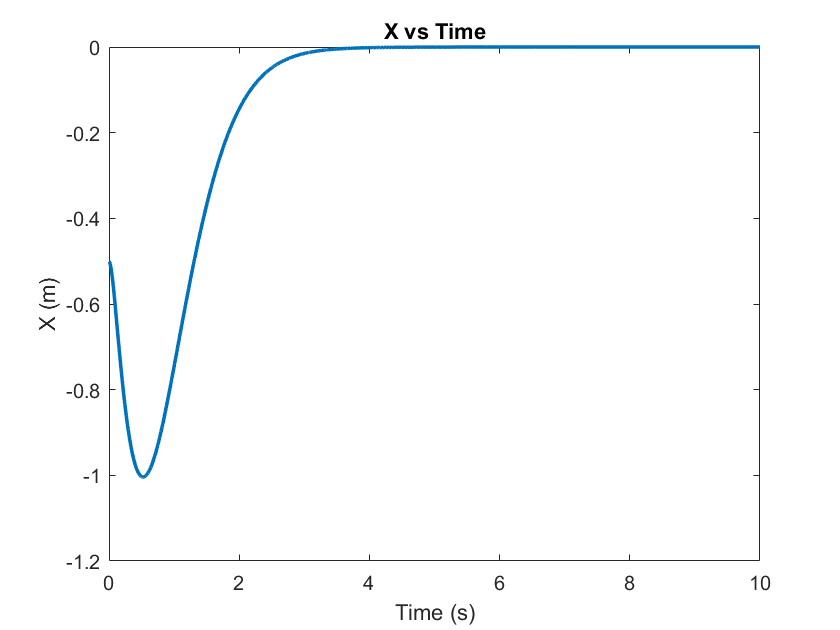
\includegraphics[width=\linewidth]{figs/sf_lin_c2_x.png}
    \caption{Combination $\#$2 - Linear System X Output}
    \label{}
\end{figure}

\begin{figure}[!ht]
    \centering
    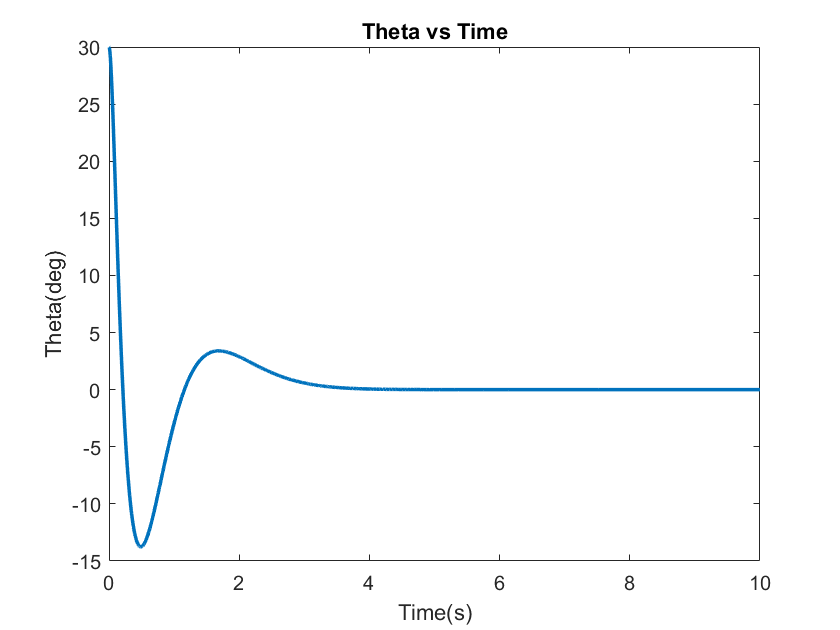
\includegraphics[width=\linewidth]{figs/sf_lin_c2_theta.png}
    \caption{Combination $\#$2 - Linear System $\theta$ Output}
    \label{}
\end{figure}

\begin{figure}[!ht]
    \centering
    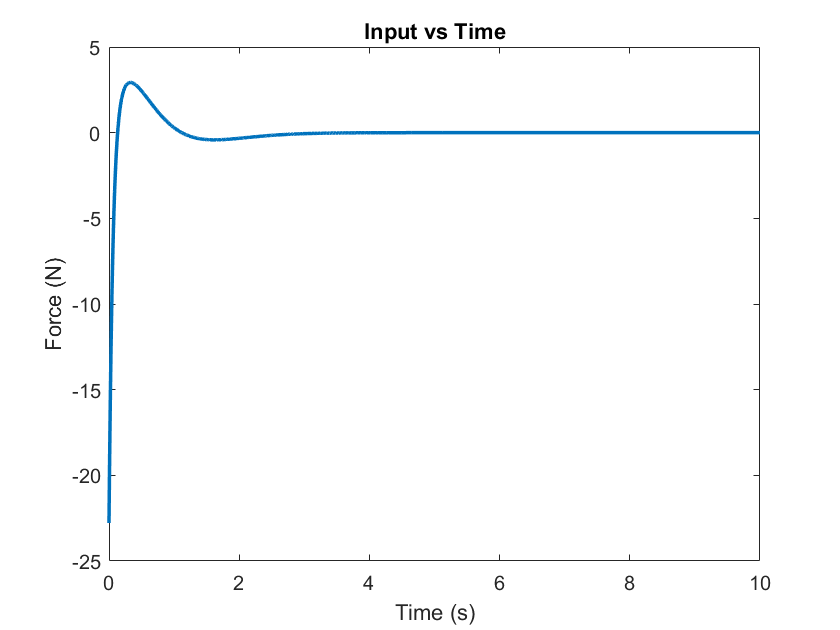
\includegraphics[width=\linewidth]{figs/sf_lin_c2_input.png}
    \caption{Combination $\#$2 - Linear System Input}
    \label{}
\end{figure}

\begin{figure}[!ht]
    \centering
    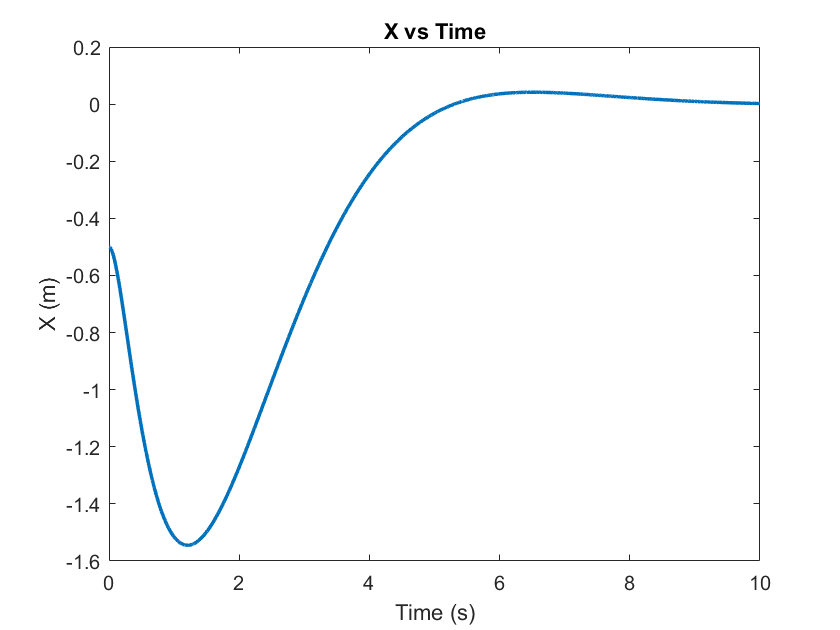
\includegraphics[width=\linewidth]{figs/sf_lin_c3_x.png}
    \caption{Combination $\#$3 - Linear System X Output}
    \label{}
\end{figure}

\begin{figure}[!ht]
    \centering
    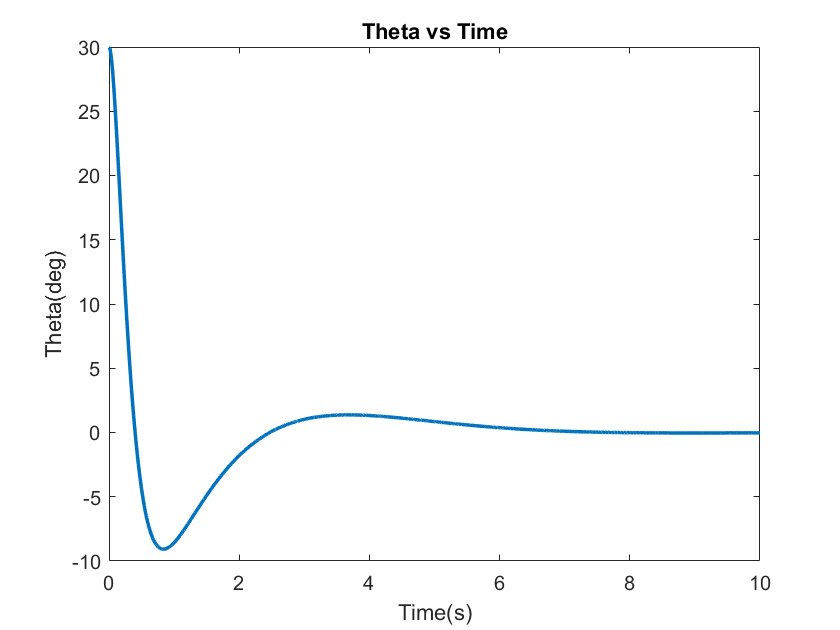
\includegraphics[width=\linewidth]{figs/sf_lin_c3_theta.png}
    \caption{Combination $\#$3 - Linear System $\theta$ Output}
    \label{}
\end{figure}

\begin{figure}[!ht]
    \centering
    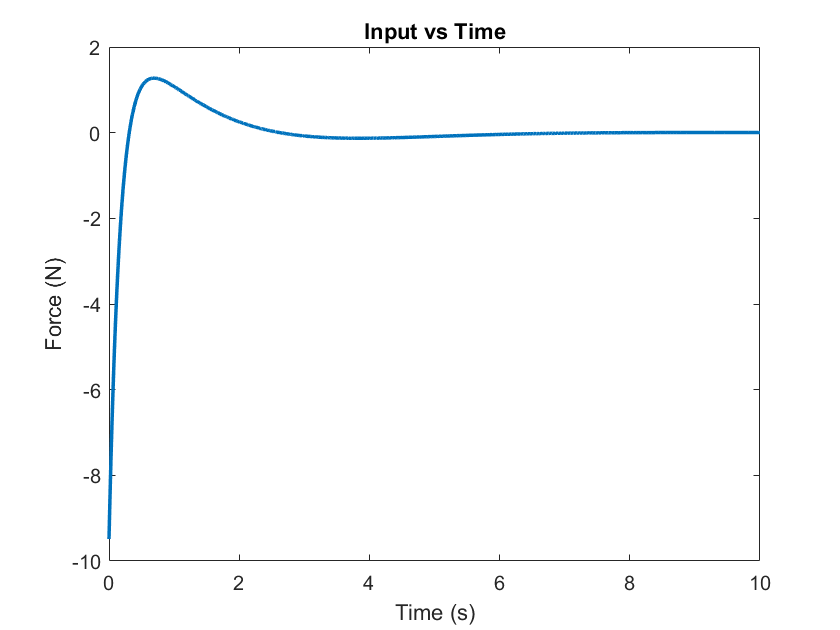
\includegraphics[width=\linewidth]{figs/sf_lin_c3_input.png}
    \caption{Combination $\#$3 - Linear System Input}
    \label{}
\end{figure}

\begin{figure}[!ht]
    \centering
    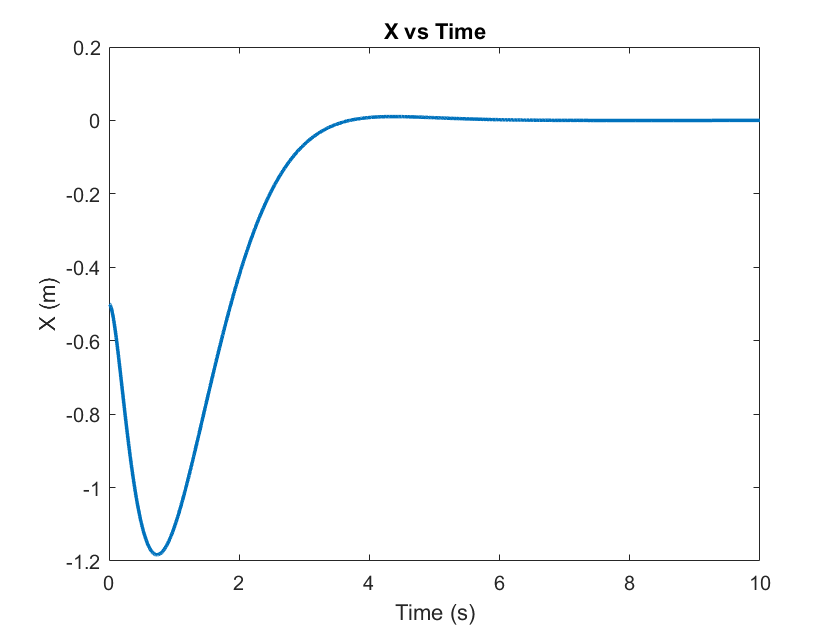
\includegraphics[width=\linewidth]{figs/sf_lin_x.png}
    \caption{Combination $\#$4 - Linear System X Output}
    \label{}
\end{figure}

\begin{figure}[!ht]
    \centering
    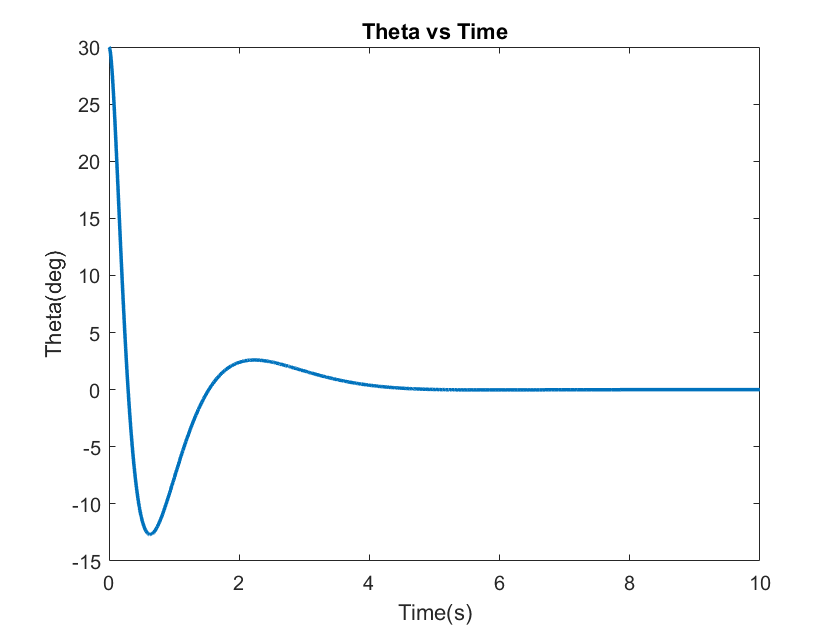
\includegraphics[width=\linewidth]{figs/sf_lin_theta.png}
    \caption{Combination $\#$4 - Linear System $\theta$ Output}
    \label{}
\end{figure}

\begin{figure}[!ht]
    \centering
    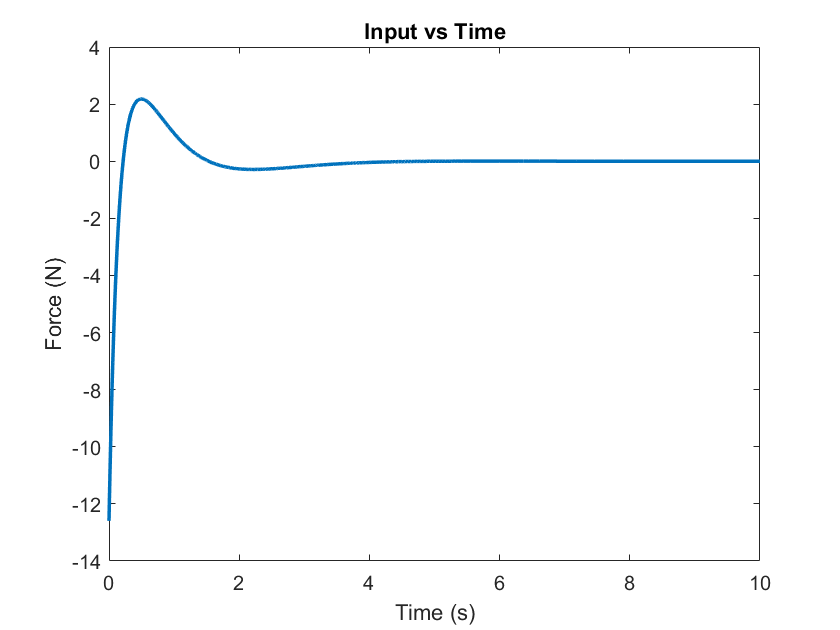
\includegraphics[width=\linewidth]{figs/sf_lin_input.png}
    \caption{Combination $\#$4 - Linear System Input}
    \label{}
\end{figure}

\begin{figure}[!ht]
    \centering
    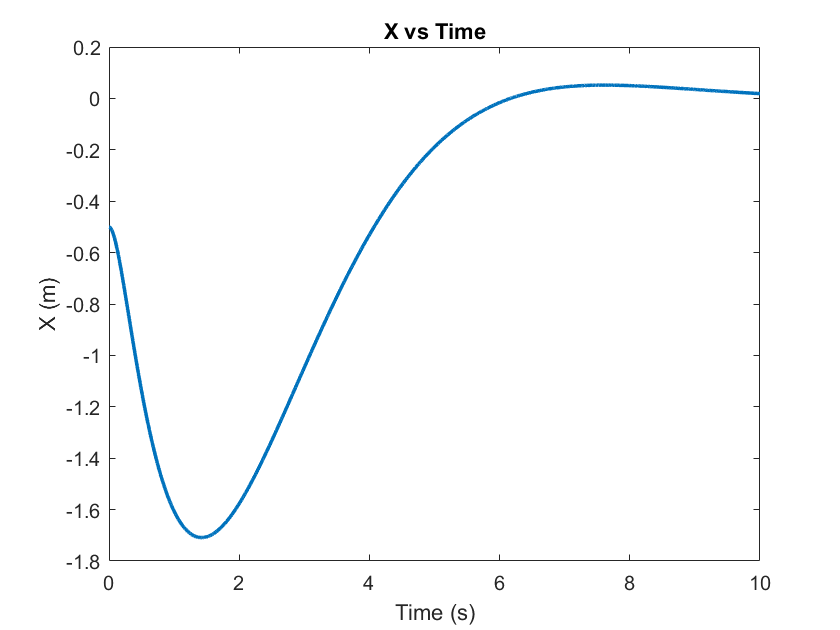
\includegraphics[width=\linewidth]{figs/sf_lin_c5_x.png}
    \caption{Combination $\#$5 - Linear System X Output}
    \label{}
\end{figure}

\begin{figure}[!ht]
    \centering
    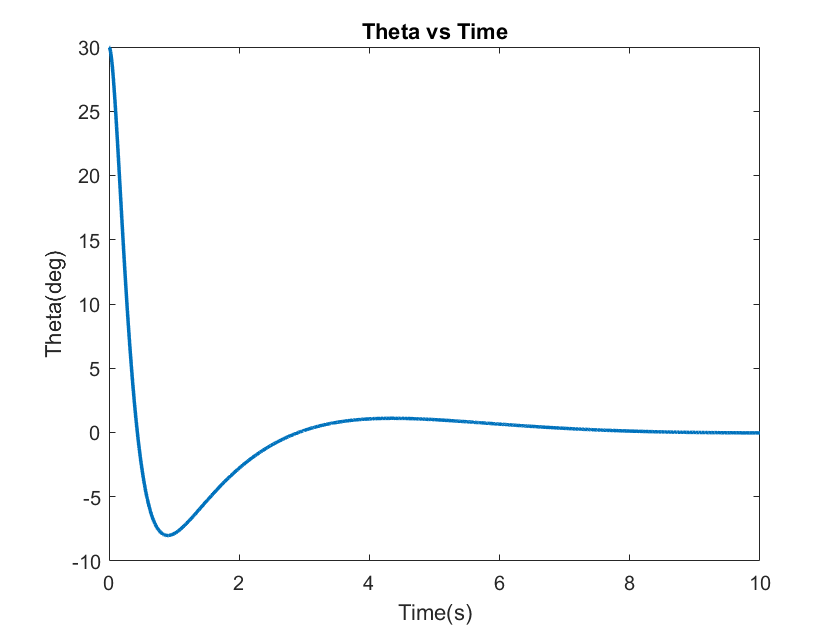
\includegraphics[width=\linewidth]{figs/sf_lin_c5_theta.png}
    \caption{Combination $\#$5 - Linear System $\theta$ Output}
    \label{}
\end{figure}

\begin{figure}[!ht]
    \centering
    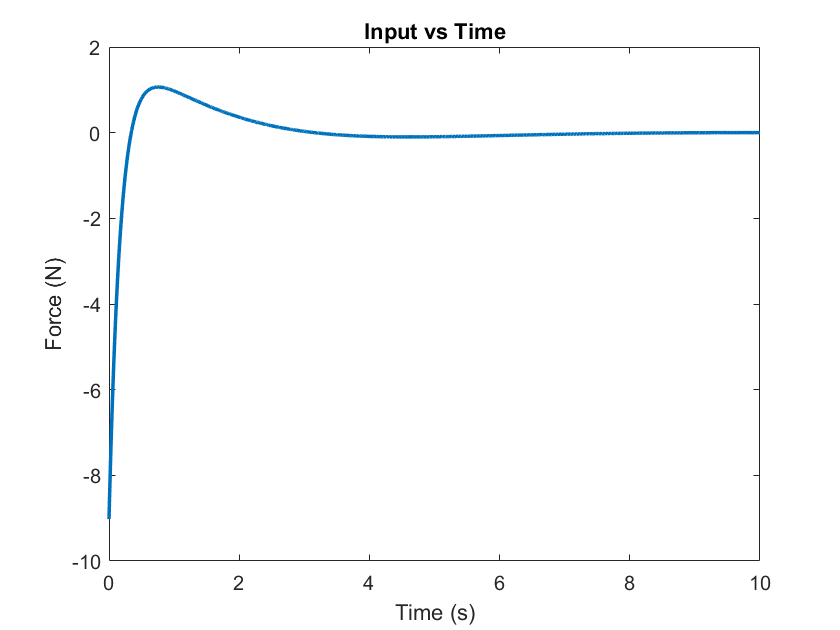
\includegraphics[width=\linewidth]{figs/sf_lin_c5_input.png}
    \caption{Combination $\#$5 - Linear System Input}
    \label{}
\end{figure}

\clearpage


Overall, increasing the values of $Q$ made the state response quicker without drastically changing the input (however it slightly increases) and decreasing $Q$ makes the response slower, but doesn't drastically change the input.  On the other hand, increasing $R$ decreased the input and made the response slower. Decreasing $R$ did the opposite. Using the modified $Q$ in Combination 1 eliminates the consideration for the derivative states which makes the response slightly slower while still being somewhat similar.

\end{document}